 % -*- root: ../main.tex -*-
\documentclass[../main.tex]{subfiles}
\begin{document}

\chapter{Les Hormones Thyroïdiennes}

% =====================================================
% ======= BEGIN - Généralités

\section{Généralités}

	La curiosité et la santé humaine sont les deux principaux catalyseurs sous-jacent au besoin de l'homme d'élargir sa connaissance en science et en biologie.
	L'historique de la biologie de la glande thyroïde et des \glspl{ht} illustre parfaitement cela.
	Dès l'antiquité en Inde et en Chine, on observait que le goitre (hypertrophie de la glande thyroïdienne) pouvait être soigné en introduisant dans l'alimentation des aliments riches en iode \citep{Niazi2011}.
	En 1656, l'anatomiste Thomas Wharton donna son nom actuel à la thyroïde sur la base de sa forme réminiscente d'un bouclier (\textit{thyreoeidês}: ``semblable à un bouclier long, scutiforme'').
	Il faudra attendre 1849 pour que le lien formel entre l'iode et la glande thyroïde se tisse.
	Les efforts se concentrèrent alors sur l'identification des composés pouvant servir de médiateur de la fonction biologique de la glande thyroïde.
	En 1895, Adolf Magnus-Levy apporta les premiers éléments de réponse en montrant que la consommation d'extrait de glande thyroïde entrainait l'augmentation du métabolisme général \citep{Magnus-Levy1895}.
	L'année suivante, E. Baumann montrait que l'iode se concentrait dans la glande thyroïde, mais pas dans les autres tissus\citep{Baumann1896}.
	\par
	En 1905, Ernest Starling utilisa pour la première fois le terme ``d'hormone'' dans une de ses conférences, ouvrant ainsi la voie à l'endocrinologie .
	Un événement important dans l'histoire des \glspl{ht} est la mise en évidence en 1912 par Gudernatch de leur fonction dans la métamorphose des amphibiens \citep{Gudernatsch1912}.
	C'est en effet en donnant des extraits de glande thyroïde à des têtards et en observant l'induction de leur métamorphose qu'il en déduisit que cet organe produit les \glspl{ht}.
	Puis, Edward C. Kendal isolait en 1915 la thyroxine et cette dernière fut synthétisée en laboratoire en 1926 par Charles R. Harington.
	La T3 qui est considérée comme la forme la plus active fut mise en évidence plus tardivement \citep{Gross1952,Roche1952}.
	Depuis, de nombreuses découvertes ont éclairé la fonction biologique des \glspl{ht}, leurs mécanismes d'action, leur métabolisme par les désiodases et le contrôle de leur production par l'axe hypothalamo-hypophyso-thyroïdien.

	% BOTTOM caption
% ------------------------
\begin{figure}[!htb]
\centering
\vspace{1\baselineskip}
\includegraphics[width=\textwidth]
% ------------------------
%
% SIDE caption
% ------------------------
%\begin{SCfigure}[\sidecaptionrelwidth][!htbp]
%\centering
%\vspace{1\baselineskip}
%\includegraphics[width=0.5\textwidth]
% ------------------------
%
% Main information
% ===========================================================
{Figures/thyroid-gland/thyroid-gland.pdf}
\caption[Anatomie et histologie de la glande thyroïde]
{
Anatomie et histologie de la glande thyroïde.
A) La glande thyroïde est située ventralement dans le cou, sous le cartilage thyroïde et autour de la trachée et de l'œsophage.
Elle est composée de deux lobes (droit et gauche) reliés par l'isthme.
Sur la face dorsale de la glande se situent les glandes para-thyroïdes.
B) Trois principales structures histologiques sont impliquées dans la production des \glspl{ht}.
Les follicules (F) sont des structures sphériques entourées d'une couche épithéliale de cellules folliculaire (thyréocytes; T).
Le lumen de ces follicules, composé de colloïde (C), sert de lieu de stockage aux précurseurs nécessaires à la synthèse des \glspl{ht} par les thyréocytes, en particulier de thyroglobuline.
Les cellules para-folliculaires (CPF) sont réparties dans les espaces interstitiels entre les follicules, et secrète la calcitonine.
Images tirées des cours en ligne de l'université du Connecticut et du département de biologie de l'université du Massachusetts Amherst.
}
\label{fig:thyroid-gland}
% ===========================================================
%
% BOTTOM caption
% ------------------------
\end{figure}
% ------------------------
%
% SIDE caption
% ------------------------
%\end{SCfigure}
% ------------------------
%
%
%\missingfigure{Make a figure}

	Les \glspl{ht}, synthétisées dans la glande thyroïde (\autoref{fig:thyroid-gland}~A) par les thyréocytes (\autoref{fig:thyroid-gland}~B), sont des hormones à la structure conservée au cours de l'évolution.
	L'analyse de génomes d'échinodermes, de chordés basaux et de vertébrés suggère que la machinerie nécessaire au métabolisme et à la signalisation thyroïdienne est un caractère ancestral des chordés, voire des deutérostomes \citep{Paris2008} (\autoref{fig:ht-tree}).

	\begin{figure}[!htb]
\centering
\vspace{1\baselineskip}
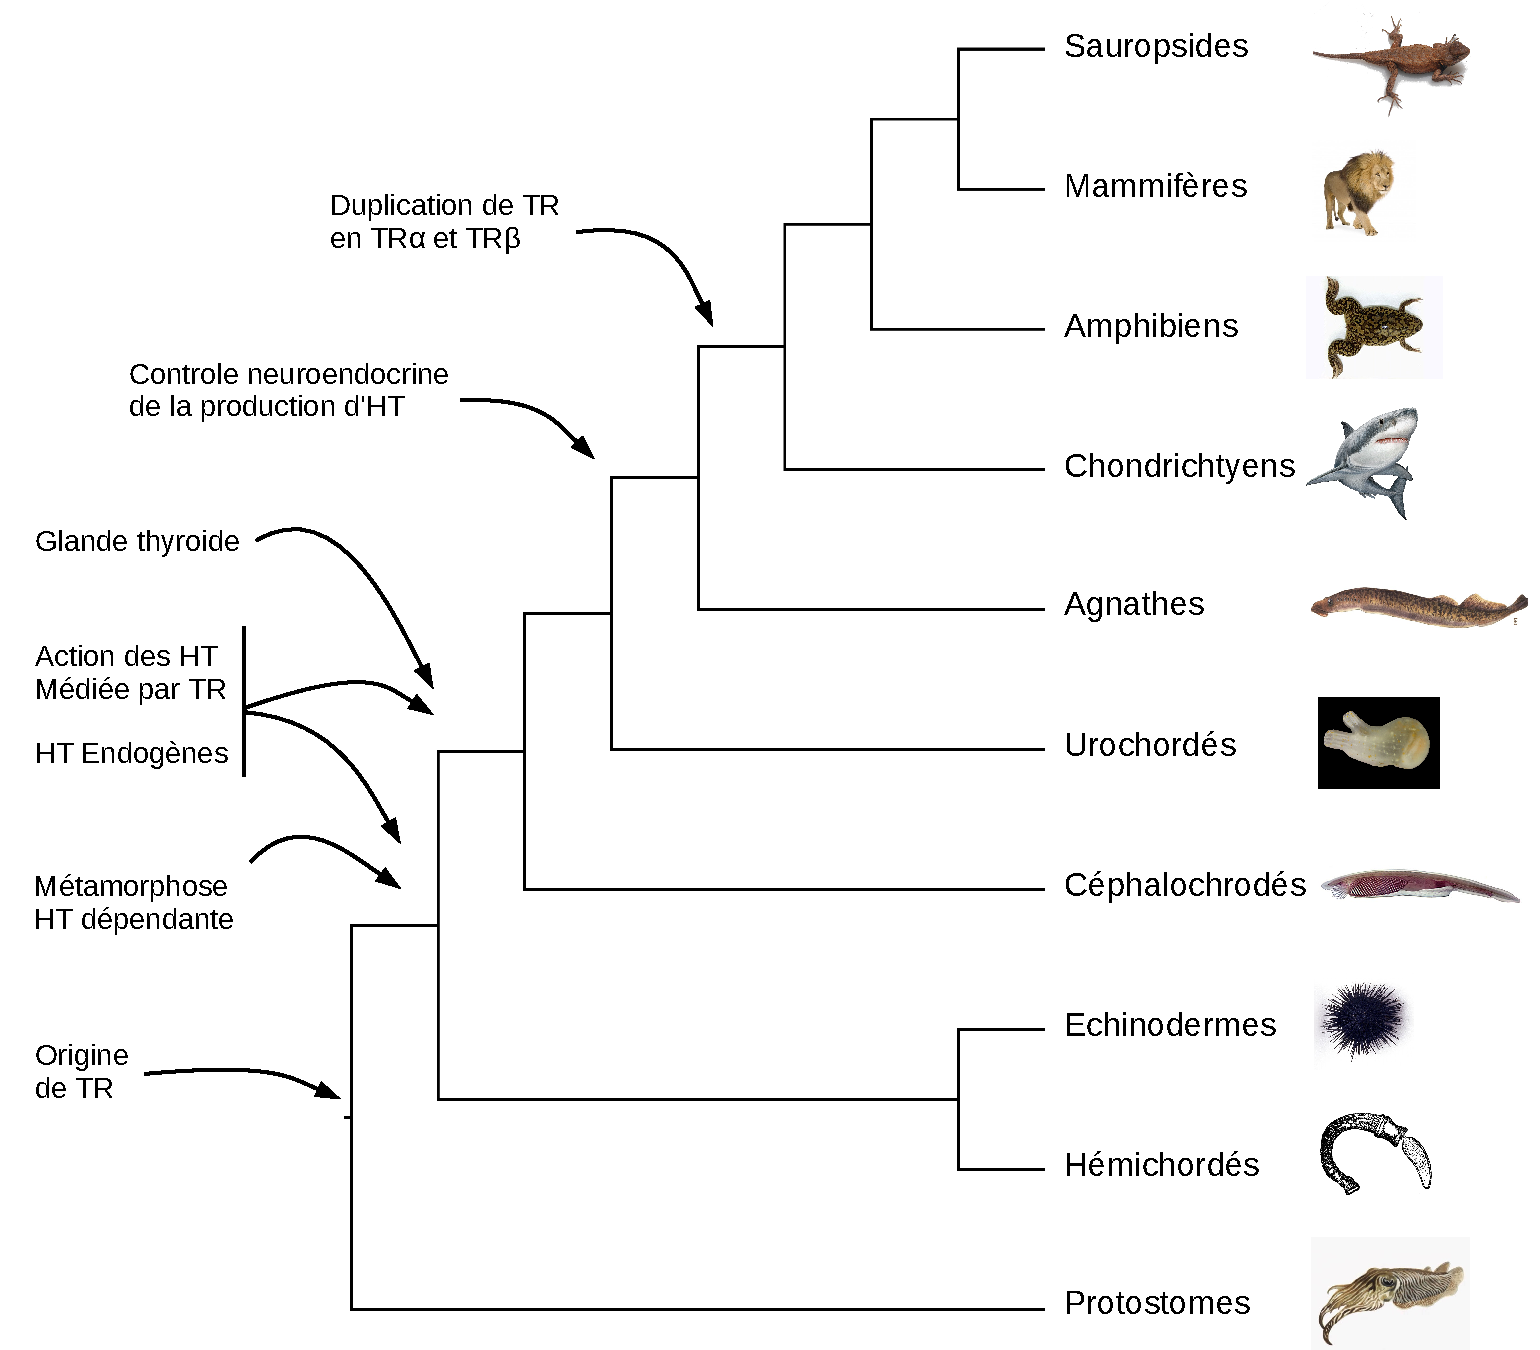
\includegraphics[width=\textwidth]
{Figures/ht-tree/ht-tree.pdf}
\caption[Évolution la signalisation thyroïdienne]
{
Les étapes principales de l'établissement de la signalisation thyroïdienne au cours de l'évolution sont représentées sur cet arbre simplifé.
Figure basée sur \citet{Paris2008}
}
\label{fig:ht-tree}
\end{figure}

	Deux rôles des \glspl{ht} ont co-évolué.
	Le premier est un rôle durant le développement post-embryonnaire.
	À la période périnatale chez les amniotes et durant la métamorphose chez les amphibiens et les autres gnathostomes non-amniotes, le taux d'\glspl{ht} circulant augmente considérablement et transitoirement.
	Chez tous ces organismes, les \gls{ht} sont cruciales dans le développement et la maturation de nombreux organes et tissus \citep{Boelaert2005}, notamment le système nerveux, le système cardiovasculaire, le système digestif, les os \citep{Wojcicka2013a}, les organes reproducteurs, les yeux ou encore les oreilles (pour revue voir \citealp{Wagner2008,Ojamaa2010}).
	Un dysfonctionnement de la signalisation thyroïdienne à cette période peut ainsi se traduire par des pathologies graves dont les effets délétères perdurent toute la vie de l'individu.
	Chez l'humain, une hypothyroïdie congénitale (le crétinisme) se traduit entre autre par un retard mental et un retard de la croissance (un faible développement des muscles squelettiques et une ossification du squelette retardée) \citep{Zimmermann2009}.
	Au contraire, une hyperthyroïdie congénitale entraîne une thyrotoxicose associée à une ossification prématurée, une croissance retardée, une arythmie cardiaque et tachycardie et dans certains cas une surdité \citep{Krude1997}.
	\par
	Le second rôle des \glspl{ht} relève essentiellement de la régulation du métabolisme et de l'homéostasie générale (voir \autoref{subsec:ht-metabolism}).
	Les \glspl{ht} agissent sur de nombreux tissus cibles: \gls{snc}, foie \citep{Weitzel2003}, gonades \citep{Wagner2008}, muscles (squelettiques et cardiaque), squelette, tissu adipeux (\autoref{fig:ht-general-actions}).
	Via leurs effets sur le \gls{sns}, elles vont également avoir un effet important sur l'ensemble des viscères et des glandes endocrines.
	%Les \glspl{ht} sont essentielles dans la régulation de l'activité cardiaque (rythme et intensité des contraction) en régulant entre autre l'expression de gènes codant pour une myosine cardiaques et une \gls{atp}ase, ou encore en contrôlant le transport d'acides aminée, d'ions et de sucres à travers la membrane plasmique \citep{Klein2007}.
	Certains des effets représentent une autre facette de leur rôle développemental.
	Le squelette par exemple, est un organe particulièrement dynamique et son remodelage permanent est en partie contrôlé par les \glspl{ht} \citep{Greenspan1999,Wojcicka2013a}.
	Le rôle des \glspl{ht} sur le métabolisme peut être fortement influencé par des facteurs environnementaux, comme la température ambiante ou la quantité d'énergie assimilée.
	Elles ont ainsi un rôle crucial dans la thermogenèse \citep{Bianco2005}.
	En effet, elles régulent d'une part le catabolisme à l'échelle cellulaire et d'autre part les voix oxydatives mitochondriales. La présence et l'activité des graisses brunes sont associés au statut thyroïdien chez la souris \citep{Bianco2005}.

	% ONE columns
% ------------------------
\begin{figure}[!htbp]
\centering
\vspace{1\baselineskip}
\includegraphics[width=\textwidth]
% ------------------------
%
% TWO columns
% ------------------------
%\begin{SCfigure}[\sidecaptionrelwidth][!htbp]
%\centering
%\vspace{1\baselineskip}
%\includegraphics[width=0.5\textwidth]
% ------------------------
%
% Main information
% ===========================================================
{Figures/ht-general-actions/ht-general-actions.pdf}
\caption[Principales fonctions biologiques impliquant les hormones thyroïdiennes]
{
Principales fonctions biologiques impliquant les hormones thyroïdiennes.
a. Glande thyroïde.
b. Métabolisme des os.
c. Contraction musculaire.
d. Système nerveux sympathique.
e. Système nerveux central.
f. Audition.
g. Vue.
h. Système cardiovasculaire.
i. Fonctions hépatiques.
j. Fonctions rénales.
k. Digestion.
l. Reproduction.
m. Thermogenèse.
n. Métabolisme
}
\label{fig:ht-general-actions}
% ===========================================================
%
% ONE columns
% ------------------------
\end{figure}
% ------------------------
%
% TWO columns
% ------------------------
%\end{SCfigure}
% ------------------------
%
%
%\missingfigure{Make a figure}

% ======= END - Généralités
% =====================================================

% :::::::::::::::::::::::::::::::::::::::::::::::::::::

% =====================================================
% ======= BEGIN - Métabolisme des HT

\section{Métabolisme et transport des hormones thyroïdiennes}\label{subsec:ht-metabolism}

	% -------------------------------
	% +++ BEGIN - Synthèse des HT

	\subsection{Synthèse des hormones thyroïdiennes}

		Les \glspl{ht} sont des hormones basées sur la tyrosine et contenant de un à quatre atomes d'iodes.
		Elles concentrent ainsi la quasi-totalité de l'iode au sein d'un organisme.
		Leur production sous forme de \gls{t4} et de \gls{t3} est un processus se déroulant en plusieurs étapes :
		\begin{enumerate}
			\item La thyroglobuline est synthétisée par les thyréocytes, des cellules folliculaires de la glande thyroïde et stockée dans la substance colloïde (\citealp{Lissitzky1981}; \autoref{fig:thyroid-gland}~B).
			\item Les groupements phénol des résidus tyrosine de la thyroglobuline sont ensuite mono- ou di- iodés de façon covalente par l'enzyme thyroperoxidase, formant ainsi des résidus \glspl{mit} et \glspl{dit}.
			\item La \gls{t4} est formée par condensation de deux résidus \glspl{dit}, tandis que la \gls{t3} est formée par condensation d'un résidu \gls{mit} et un résidu \gls{dit}.
			\item La stimulation des thyréocytes par la \gls{tsh} engendre l'endocytose de la colloïde et la protéolyse des thyroglobulines iodées afin d'en libérer la \gls{t3} et la \gls{t4} (pour revue \citealp{Rousset2003}).
			Celles-ci sont relarguées liées à des protéines de transport (voir \autoref{subsec:ht-transport}) dans la circulation sanguine afin d'agir sur les tissus cibles.
		\end{enumerate}

	% +++ END - Synthèse des HT
	% -------------------------------
	% +++ BEGIN - Transport des HT

	\subsection{Transport des hormones thyroïdiennes}\label{subsec:ht-transport}

		\subsubsection{Transporteurs sanguins}
			Les \glspl{ht} sont des molécules hydrophobes relativement peu stables.
			Afin de les stabiliser et d'augmenter leur temps de demi-vie, la quasi-totalité des \glspl{ht} plasmatiques sont liées à des protéines de transport, dont les plus importantes sont la \gls{ttr} \citep{Palha2002}, l'albumine et la \gls{tbg} \citep{Schussler2000}.
			Cette dernière lie avec une grande affinité la majorité de la \gls{t3} et \gls{t4} circulante.
			Malgré sa faible concentration plasmatique, elle reste souvent peu saturée.
			L'albumine, au contraire, a une affinité moindre, mais est présente en grandes quantités dans la circulation sanguine, ce qui lui confère également un rôle majeur.
			Au niveau des tissus cibles, les \glspl{ht} sont découplées de leurs transporteurs car seule la fraction libre peut pénétrer les cellules \citep{Ekins1994}.

		\subsubsection{Transporteurs membranaires}
			Jusque dans les années 1970, il était supposé que les \glspl{ht} pénétraient la membrane cytoplasmique des cellules cibles par simple diffusion. Cette hypothèse se basait sur la nature lipophile des \glspl{ht}.
			Les premiers indices d'un transport actif des \glspl{ht} à travers la membrane ont été fournis par \citet{Christensen1954}, puis par \citet{Rao1976}. Plusieurs études indépendantes ont depuis mis en évidence une pléthore de transporteurs, la majorité étant \gls{Na}- et \gls{atp}-dépendants. Les mieux décrits sont les \glspl{oatp} et les \glspl{mct}.
			\par
			Les \glspl{oatp} représentent une grande famille de protéines de transport \gls{Na}-indépendant multispécifiques de composés amphiphatiques organiques.
			Cette multispécificité de substrat souligne l'importance que les \glspl{oatp} possèdent dans un contexte de détoxification.
			Plus de 40 membres ont été caractérisés à ce jour, chacun d'eux étant plus ou moins \glspl{ht}- et tissu-spécifique.
			En particulier, \gls{oatp}1C1 possède une forte affinité pour la \gls{t4} et la \gls{rt3}.
			\par
			Les \glspl{mct} doivent leur nom au fait qu'elles ont initialement été caractérisées comme assurant le transport de lactate, pyruvate et de corps cétoniques.
			Ce sont des symporteurs de protons et leur efficacité est en conséquence dépendante du pH.
			Parmi les 14 \glspl{mct} identifiées à ce jour, seules \gls{mct}8 et \gls{mct}10 ont été décrites comme des transporteurs très spécifiques des \glspl{ht} \citep{Friesema2003,Friesema2008}.
			%Curieusement, les souris K.O. pour \gls{mct}8 ne présentent pas de retard mentaux imputables à un développement cérébral anormal comme c'est le cas chez l'humain.
			%Ceci suggère une redondance de la fonction de certaines \glspl{mct} espèce-spécifique.

	% +++ END - Transport des HT
	% -----------------------------------
	% +++ BEGIN - Métabolisme local des HT

	\subsection{Contrôle de la production et de la disponibilité des hormones thyroïdiennes}\label{subsec:th-prod-control}
		Chez l'humain au sein des tissus, la \gls{t4} est 3 à 5 fois plus abondante que la \gls{t3} \citep{Laurberg1984}. Elles agissent au niveau de nombreux tissus cible et jouent un rôle important dans l'homéostasie générale.
		La quantité d'\glspl{ht} dans l'organisme, qui se doit d'être finement régulée, est ainsi modulée à deux niveaux.

		\subsubsection{L'axe \gls{hpt}}\label{subsubsec:hpt}
			La synthèse de \gls{t3} et \gls{t4} et la sécrétion de thyroglobuline dans le colloïde par les thyréocytes sont déclenchées par la \gls{tsh} \citep{Vagenakis1973}.
			Cette dernière est une hormone et une glycoprotéine secrétée par les cellules thyréotropes de l'anté-hypophyse.
			Sa production et sa sécrétion sont activées par la \gls{trh} \citep{Halasz1965}.
			La \gls{trh} est produite par les neurones médians de la zone para-ventriculaire de l'hypothalamus.
			L'axe  \gls{hpt} intègre ces trois organes dans une boucle de rétro-contrôle négatif par la \gls{t3} et la \gls{t4}, ces dernières inhibant la synthèse de \gls{tsh} \citep{Larsen1982} et de \gls{trh} \citep{Koller1987} (\autoref{fig:hpt}).
			Ce type de régulation vise à maintenir des niveaux d'\glspl{ht} constants.

			% BOTTOM caption
% ------------------------
\begin{figure}[!htbp]
\centering
\vspace{1\baselineskip}
\includegraphics[width=\textwidth]
% ------------------------
%
% SIDE caption
% ------------------------
%\begin{SCfigure}[\sidecaptionrelwidth][!htbp]
%\centering
%\vspace{1\baselineskip}
%\includegraphics[width=0.5\textwidth]
% ------------------------
%
% Main information
% ===========================================================
{Figures/hpt/hpt.pdf}
\caption[L'axe hypothalamo-hypophyso-thyroïdien]
{
La synthèse et la sécrétion d'\glspl{ht} par la thyroïde sont stimulées par la \gls{tsh}, produite au niveau de l'antéhypophyse.
La stimulation de la synthèse de la \gls{tsh} est elle-même sous le contrôle de la \gls{trh}, produite par l'hypothalamus.
La \gls{t3} et la \gls{t4} exercent un rétro-contrôle négatif sur ce système en inhibant la synthèse de \gls{tsh} et de \gls{trh}.
}
\label{fig:hpt}
% ===========================================================
%
% BOTTOM caption
% ------------------------
\end{figure}
% ------------------------
%
% SIDE caption
% ------------------------
%\end{SCfigure}
% ------------------------
%
%
%\missingfigure{Make a figure}

		\subsubsection{Les désiodases}
			Alors que l'axe \gls{hpt} permet la régulation des niveaux systémiques en \glspl{ht}, la disponibilité locale en hormone biologiquement active est modulée directement dans les tissus cibles \citep{Bianco2006}.
			La glande thyroïde synthétise la totalité de la \gls{t4}, mais seulement 10 à 20 \% de la \gls{t3} \citep{Laurberg1984}.
			Au sein des tissus cibles, la conversion entre les différentes formes des \glspl{ht} est assurée par des enzymes spécialisées, les désiodases.

			\begin{figure}[!htbp]
\centering
\vspace{1\baselineskip}
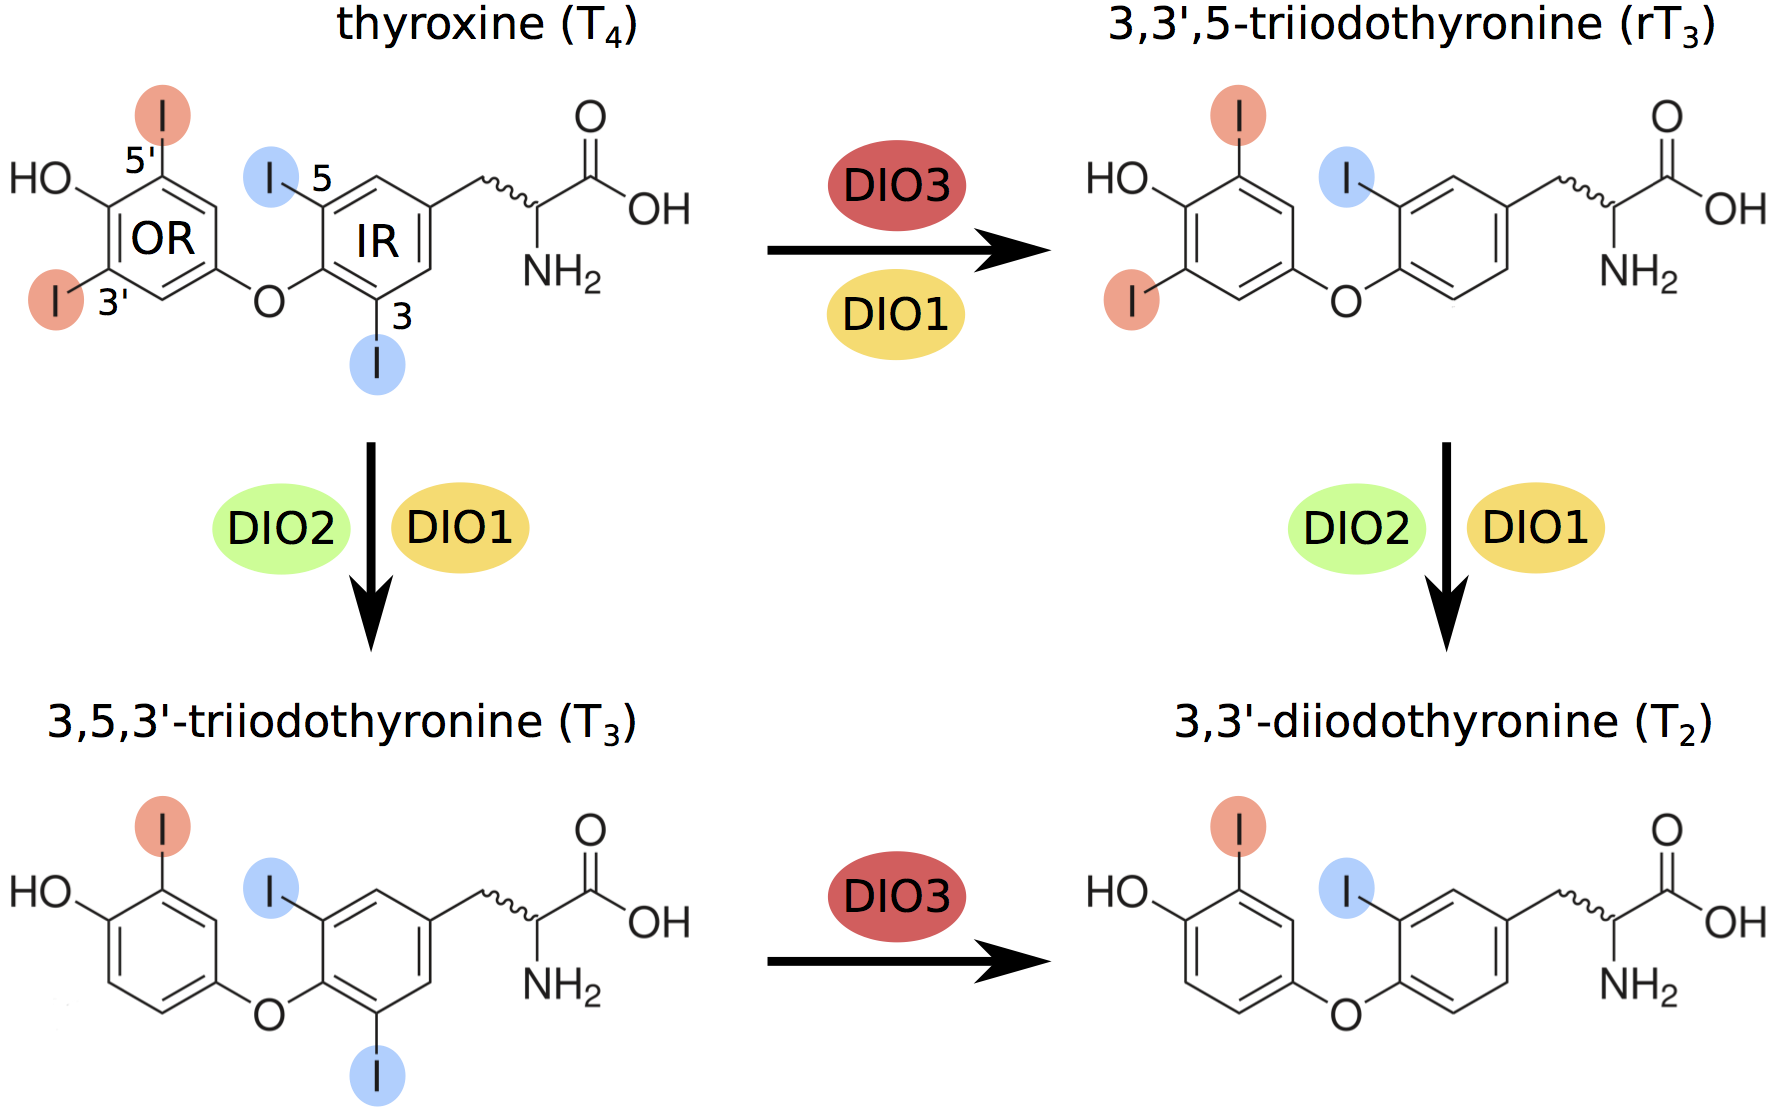
\includegraphics[width=\textwidth]
{Figures/ht-dio/ht-dio.png}
\caption[Réactions de désiodation de base]
{
Les réactions catalysées par les désiodases retirent les atomes d'iode (sphères rouges et bleues) du cycle externe (groupement phénol, positions 3' et 5', sphères rouges) ou du cycle interne (groupement tyrosine, positions 3 et 5, sphères bleues).
Ces voies peuvent activer la \gls{t4} en la transformant en \gls{t3} (\textit{via} \gls{dio1} ou \gls{dio2}) ou en l'empêchant d'être activée en la convertissant en la forme métaboliquement inactive \gls{rt3} (\textit{via} \gls{dio1} ou \gls{dio3}). La \gls{t2} est un produit commun aux deux voies, peu actif et rapidement métabolisé.
}
\label{fig:ht-dio}
\end{figure}

			Les désiodases sont des sélénoprotéines peroxydases, catabolisant la substitution d'un atome d'iode par un atome d'hydrogène.
			La \gls{t3} est majoritairement obtenue au niveau des tissus cibles par \gls{ord} en position $5\prime$ de la pro-hormone \gls{t4}.
			Cette réaction irréversible est assurée en partie par la \gls{dio2} (pour revue \citealp{Williams2011}) et correspond à une activation des \glspl{ht} (\autoref{fig:ht-dio}).
			La \gls{dio3} peut également exercer sur la \gls{t3} et la \gls{t4} une activité \gls{ird} en position 5.
			Les métabolites qui en résultent, respectivement la \gls{rt3} et la \gls{t2}, sont très biologiquement actifs (bien qu'une action de la \gls{t2} passant par \gls{tr} ait été suggérée \citealp{Mendoza2013}).
			Ceci fait de la \gls{dio3} une enzyme essentiellement inactivante (\autoref{fig:ht-dio}).
			La première désiodase à avoir été caractérisée, la \gls{dio1}, peut aussi bien activer les \glspl{ht} (\gls{t4} à \gls{t3}) qu'empêcher leur activation (\gls{t4} à \gls{rt3}).
			Compte tenu que son substrat préférentiel est la \gls{rt3}, la \gls{dio1} semble avoir un rôle important dans la clairance des \glspl{ht} \citep{Maia2011}, le recyclage de l'iode contenu dans les métabolites des \glspl{ht} \citep{Schneider2006} et la biosynthèse de thyronamines.
			Ces dernières sont des composés dont les effets peuvent s'opposer à ceux des \glspl{ht}, en particulier dans le contrôle de l'activité cardiaque et de la thermogenèse \citep{Scanlan2004}.
			\par
			De part leur importance dans le cadre de la régulation de la quantité d'\glspl{ht} actives, elles sont à l'origine de nombreux syndromes métaboliques (\autoref{tab:desiodases})

			\begin{sidewaystable}[!htbp]
{
\footnotesize
\newcolumntype{L}{>{\raggedright\arraybackslash}X}
\begin{tabularx}{\textwidth}{L L L L}

\toprule

\textbf{Paramètre} &
	\textbf{\gls{dio1}} &
	\textbf{\gls{dio2}} &
	\textbf{\gls{dio3}} \\

\midrule

\textbf{Propriétés biochimiques} & ~ & ~ & ~ \\
	Substrats préférentiels (position) &
		\gls{rt3} (5') &
		\gls{t4} \gls{rt3} &
		\gls{t4} \gls{t3} \\
	Demi-vie &
		Plusieurs heures &
		\~ 20 minutes &
		Plusieurs heures \\
	Localisation sub-cellulaire &
		Membrane plasmique &
		Réticulum endoplasmique &
		Membrane plasmique \\
\textbf{Tissus préférentiels} & ~ & ~ & ~ \\
	~ &
		Foie, rein &
		Système nerveux central, hypophyse, tissu adipeux brun, placenta &
		Placenta, système nerveux central \\
\textbf{Réponse à des taux élevés de \gls{t3} et \gls{t4}} & ~ & ~ & ~ \\
	Transcriptionelle &
		$\uparrow \uparrow$ &
		$\downarrow$ &
		$\uparrow \uparrow$ \\
	Post-traductionelle &
		? &
		$\downarrow \downarrow \downarrow$ (Ubiquitination) &
		? \\
\textbf{Régulations physiologiques} & ~ & ~ & ~ \\
	Induction &
		\gls{t3} &
		Froid, suralimentation, catécholamines, acides biliaires, cAMP &
		\gls{t3}, lésions tissulaires, TGF , FGF, EGF, PDGF, activateurs de ERK \\
	Répréssion &
		Jeûne, maladie &
		\gls{t3}, \gls{t4}, Hedgehog &
		\glspl{gc}, hormones de croissance \\
\textbf{Rôles physiologiques} & ~ & ~ & ~ \\
	~ &
		Clairance de la \gls{rt3} &
		Thermogenèse, développement, fournit la \gls{t3} intracellulaire, source majeure de \gls{t3} plasmatique &
		Développement, clairance de \gls{t3} et \gls{t4}, empêche l'accumulation de \gls{t3} intracellulaire \\
\textbf{Rôles dans des contextes pathologiques} & ~ & ~ & ~ \\
	~ &
		Source principale de \gls{t3} circulante chez les patients hyperthyroïdiens &
		? &
		Hypothyroïdisme "consommant", clairance de la \gls{t3} et la \gls{t4} accrue chez les femmes enceintes \\
		
\bottomrule

\end{tabularx}
}
\caption[Principales caractéristiques des désiodases]
{
Principales caractéristiques des désiodases. Adapté de \citet{Bianco2006}
}
\label{tab:desiodases}
\end{sidewaystable}

		\subsubsection{La conjugaison}
			Les \glspl{ht} peuvent être conjuguées (sulfonylation et glucuronidation) au niveau du résidu hydroxyle du cycle externe.
			Ces réactions sont particulièrement associées à la détoxification de xénobiotiques et participent à augmenter leur solubilité dans l'eau.
			Dans le contexte des \glspl{ht}, ces processus peuvent participer à leur clairance et élimination.
			\par
			La glucuronidation des \glspl{ht} est assurée par les enzymes hépatiques UDP-glucuronyl-transférases, ce qui facilite leur excrétion \textit{via} la bile \citep{Visser1996}.
			Une partie des \glspl{ht} conjuguées peut être réutilisée par l'organisme par hydrolyse du groupement glucuronide.
			Certains tissus semblent stocker les \glspl{ht} sous forme conjuguée, suggérant que la glucuronidation puisse représenter un niveau de régulation supplémentaire de l'action des \glspl{ht} \citep{VanderHeide2007}.
			\par
			La sulfonylation, quant à elle, affecte les réactions de désiodation des \glspl{ht}.
			En effet, cette réaction contribue à inhiber les actions de \gls{dio2} et \gls{dio3}, tout en favorisant l'activité \gls{ord} de \gls{dio1} \citep{Visser1990}.
			Les métabolites sulfonylés des \glspl{ht} sont rapidement dégradés, faisant de cette réaction un mécanisme de protection contre des niveaux toxiques d'\glspl{ht}.
			Dans des cas pathologiques de type hypothyroïdie associés à une faible activité de \gls{dio1}, la \gls{t3} sulfonylée n'est pas dégradée et constitue une réserve mobilisable d'\glspl{ht} et d'iode (pour revue, voir \citealp{Visser1994}).

		% +++ END - Métabolisme local des HT
		% --------------------------------------

% ======= END - Métabolisme des HT
% =====================================================

% :::::::::::::::::::::::::::::::::::::::::::::::::::::

% =====================================================
% ======= BEGIN - Méchanismes d'action des HT

\section{Mécanismes d'action des hormones thyroïdiennes}

	Les premiers indices des effets des hormones sur la transcription furent apportés dans les années 1960 par l'observation de renflements (``puffs'') de chromosomes polytènes lors d'un traitement aux ecdysteroïdes (hormones de la métamorphose et de la mue chez les insectes) \citep{Clever1960}.
	Dans les années 1963, J.R. Tata montrait que les \glspl{ht} favorisaient la synthèse d'\gls{rna} conjointement à l'augmentation du métabolisme cellulaire.
	Pendant les années 1970, les travaux de \citet{Samuels1973} ont participé à l'identification de sites protéiques de liaisons aux \glspl{ht} retrouvés dans des fractions nucléaires. Il a donc été supposé que les \glspl{ht} agissaient via un ou plusieurs récepteurs spécifiques présents dans le noyau.

	% -------------------------------
	% +++ BEGIN - Récépteurs aux HT

	\subsection{Les récepteurs aux hormones thyroïdiennes, membres de la famille de récepteurs nucléaires}\label{subsubsec:TR}

		\subsubsection{Propriétés des récepteurs nucléaires}
			Les \glspl{rn} sont des facteurs de transcription caractérisés par leur localisation nucléaire (au moins transitoire) nécessaire à leur action sur la régulation de l'expression de gènes cibles.
			Les \glspl{rn} sont en général activés par la liaison à un ligand, souvent une petite molécule lipophile.
			Il existe cependant des \glspl{rn} qualifiés d'orphelins pour lesquels aucun ligand n'a été mit en évidence (pour revue, \citealp{Giguere1999}) et dont l'activation passerait directement par des modifications post-traductionnelles.
			La liaison du ligand (et/ou les modifications post-traductionnelles) entraîne en un changement de conformation du récepteur qui modifie sa compétence à lier l'\gls{dna} et/ou à recruter des complexes co-régulateurs.
			Les \glspl{rn} agissent souvent (mais pas exclusivement) en formant des homomères ou des hétéromères avec d'autres \glspl{rn}.
			Ils modulent tous l'expression de gènes cibles en se fixant à l'\gls{dna} au niveau de séquences \textit{cis}-régulatrices, les ``éléments de réponse''.
			Ces derniers sont composés de un ou deux demi-sites caractérisés par trois paramètres :
			\begin{itemize}
				\item Une séquence canonique d'un demi-site de 4 à 8 \glspl{pb}
				\item L'orientation des deux demi-sites : répétition directe, palindrome ou palindrome inversé.	
				\item Le nombre de paire de bases séparant les deux demi-sites.
			\end{itemize}

		\subsubsection{Classification des récepteurs nucléaires}
			Les \glspl{rn} peuvent être classés en 7 sous-familles selon la similitude de séquence de leurs domaines de liaison à l'\gls{dna} et au ligand \citep{Laudet1997,Committee1999}.
			Une étape indispensable à cette mesure réside dans la connaissance et la caractérisation de leur séquence.
			Dans les années 1980, de nombreux travaux ont mené à la caractérisation de plusieurs de ces \glspl{rn}.
			En particulier, le \gls{gr} et le \gls{er} ont été clonés sur la base de leur similitude de séquence avec \gls{verbA} \citep{Hollenberg1985, Green1986}.
			Les autres \glspl{rn} ont, pour la plupart, été caractérisés selon une approche similaire.
			De façon indirecte cette classification discrimine au moins partiellement leur modalités de liaison à l'\gls{dna}, de dimérisation et le type de ligand qui les active:

			\paragraph{Sous-famille 1: famille des récepteurs aux hormones thyroïdiennes}
				Les \glspl{rn} de la sous-famille 1 sont séquestrés dans le noyau même en absence de ligand, souvent sous forme hétérodimérique avec \gls{rxr}.
				Ils interagissent alors avec des complexes co-répresseurs afin de réprimer l'expression de gènes cibles.
				En présence de ligand, leur conformation change et ils recrutent des complexes co-activateurs pour induire l'expression de gènes cibles.
				Ce groupe rassemble \gls{tr}, \gls{rar}, \gls{vdr}, \gls{ppar}, ainsi que des \glspl{rn} orphelins reliés aux rétinoïdes. Ils se fixent en général au niveau de \glspl{dr4}.

			\paragraph{Sous-famille 2: famille des récepteurs aux rétinoïdes X}
				La sous-famille 2 regroupe \gls{rxr}, \gls{couptf} et \gls{hnf4}.
				Sauf pour \gls{rxr}, ils se lient à l'\gls{dna} préférentiellement au niveau de répétitions directes sous forme d'homodimères.

			\paragraph{Sous-famille 3: famille des récepteurs stéroïdiens}
				Les \glspl{rn} de la sous-famille 3 lient des hormones stéroïdes, dont les \glspl{gc}, les \glspl{mc} et les hormones sexuelles. Ces \glspl{rn} sont en général séquestrés dans le cytoplasme par des protéines chaperonnes comme \gls{hsp90} en absence de ligand, transloqués dans le noyau sous forme d'homodimères en présence de ligand et se lient préférentiellement au niveau de \glspl{ir3}.

			\paragraph{Sous-famille 4: famille des récepteurs similaires au facteur de croissance nerveuse}
				La sous-famille Nur regroupe des \glspl{rn} orphelins similaires à \gls{ngf1b}, les deux autres membres étant \gls{nurr1} et \gls{nor1}.
				Ce sont des gènes dont l'expression est induite précocement en réponse à un stimulus et ils agissent comme facteurs de transcription activés indépendamment de la liaison à un ligand.

			\paragraph{Sous-famille 5: Récepteurs aux facteurs stéroïdogéniques}
				Cette famille regroupe \gls{sf1} et \gls{lrh1}, dont les ligands sont des phosphatidylinositols.
				Ils sont impliqués dans le développement des organes reproducteurs.
				%\citep{Lourenco2009}

			\paragraph{Sous-famille 6: Facteurs nucléaires de cellules germinales}
				Cette petite famille n'est constituée que de \gls{gcnf} qui est impliqué dans la différentiation des cellules germinales.
				Ce récepteur ne possède pas de ligand connu et se fixe à l'\gls{dna} sous forme d'homodimères.

			\paragraph{Sous-famille 0: Facteurs divers}
				La sous-famille 0 regroupe DAX1 et SHP qui ne comportent pas le domaine nécessaire à la liaison à l'\gls{dna} et jouent le rôle de répresseur d'autres \glspl{rn} en formant des hétérodimères inactifs.

		\subsubsection{Évolution des récepteurs nucléaires}
			Les \glspl{rn} sont très répandus chez tous les métazoaires, mais avec une diversité parfois hétérogène entre différentes espèces.
			Alors que 48 sont dénombrés chez l'humain \citep{Robinson-Rechavi2001}, 21 ont été dénombrés chez \textit{Drosophila melanogaster} et plus de 270 chez \textit{Caenorhabditis elegans} (pour revue, voir \citealp{Robinson-Rechavi2003}).
			Cette diversité de la répartition des \glspl{rn} chez les métazoaires s'explique par des événements locaux (duplications segmentaires ou en tandem) ou à plus grande échelle (duplications du génome entier, réarrangements chromosomiques ...).
			\par
			La multiplication des \glspl{rn}, aidée par ces événements classiques de l'évolution des génomes, s'est également accompagnée d'une diversification de leurs fonctions, en particulier via l'émergence de nouveaux couples récepteurs/ligands.
			Actuellement, deux modèles principaux proposent d'expliquer cette co-évolution.
			Le premier, l'exploitation de ligands, proposé par \citet{Thornton2001}, suggère que la diversification des \glspl{rn} (en particulier ceux de la sous-famille 3) soit basée sur l'utilisation d'intermédiaires métaboliques ou de métabolites dans les voies de biosynthèse des stéroïdes en tant que ligands.
			Le second, proposé par \citet{Escriva2006}, suggère le perfectionnement de la spécificité de liaison du ligand au \gls{rn} par mutation dans la séquence de son domaine de liaison au ligand.
			De façon intéressante, ces deux mécanismes ne sont pas mutuellement incompatibles, différentes familles de \glspl{rn} étant soumises à des pressions de sélection différentes.

		\subsubsection{Identification des récepteurs aux hormones thyroïdiennes}
			De nombreux travaux visant à élucider les mécanismes d'action des \glspl{ht} furent conduits dans les années 1980 en mesurant l'effet des \glspl{ht} et des \glspl{gc} sur la transcription du gène de la \gls{gh} .
			En 1984, Nyborg montra que l'induction de la transcription de la \gls{gh} par la \gls{t3} était dépendante d'un récepteur interagissant potentiellement avec le \gls{gr} \citep{Nyborg1984}.
			\par
			Grâce à sa similitude de séquence avec \gls{verbA}, \gls{gr} et \gls{er}, un premier \gls{tr} a pu être cloné et identifié comme \gls{cerbA} et comme correspondant à \gls{tra} \citep{Sap1986,Weinberger1986}.
			Un second \gls{tr} (\gls{trb}) a ensuite été identifié comme un autre homologue cellulaire de \gls{verbA} \citep{Thompson1987}.

		% +++ END - Récepteurs aux HT
		% -------------------------------
		% +++ BEGIN - Structure générale de TR

	\subsection{Structure des récepteurs aux hormones thyroïdiennes}\label{subsubsec:struct-tr}
		Les \glspl{tr}, comme tout autre \glspl{rn}, sont constitués de cinq domaines principaux :

		\paragraph{Le domaine A/B}
			Le domaine A/B constitue la partie N-terminale de la séquence.
			Il contient le domaine \gls{af1} dont l'action est d'assurer un taux de transcription basale.

		\paragraph{Le domaine C}
			Le domaine C contient le \gls{dbd} qui est constitué de deux structures tertiaires en ``doigts de zinc''.
			Chacune est composée de quatre cystéines autour d'un atome de zinc \citep{Evans1988}.
			Une ``boite P'' (séquence d'acides aminés EGCKG) se situe sur le premier doigt de zinc.
			Une ``boite A'' est en aval du second.
			Elle sont impliquées dans la spécificité de liaison de \gls{tr} à l'\gls{dna} au niveau de ses éléments de réponse spécifiques \citep{Nelson1993}.
			Deux surfaces de dimérisation (notamment avec \gls{rxr}) ont été décrites comme correspondant à l’arginine de la ``boite D'' sur le deuxième doigt de zinc et la ``boite T'' en aval des doigts de zinc (pour revue \citealp{Bain2007}).

		\paragraph{Le domaine D}
			Le domaine D est une région charnière qui donne des degrés de liberté dans la conformation des \glspl{rn}.
			Il favorise l'hétérodimérisation et intervient dans la spécificité de liaison à l'\gls{dna} \citep{Miyamoto2001}.
			De plus, il contient une séquence de localisation nucléaire \citep{Hamy1992a}.
			Enfin, il interagit avec certains des partenaires nécessaires à l'activité transcriptionnelle des \glspl{tr} \citep{Lin1991,Horlein1995}.

		\paragraph{Le domaine E/F}
			Il contient le \gls{lbd} et est composé de 12 hélices $\alpha$ (H1 à H12) et de quatre feuillets $\beta$ dont la ``boite I''.
			Celle-ci est constituée de répétitions d'acides aminés formant une poche hydrophobe qui permet la fixation de la \gls{t3}.
			C'est le groupe hydroxyle du ligand situé en $4\prime$ (voir \autoref{fig:ht-dio}) qui rend possible la liaison de l'hormone au \gls{lbd}.
			Il joue le rôle de donneur et accepteur d’hydrogène \citep{Dietrich1977}.
			La présence en $5\prime$ (voir \autoref{fig:ht-dio}) d'un atome autre que l'hydrogène affecte la reconnaissance du ligand, expliquant l'affinité inférieure pour la \gls{t4} ou la \gls{rt3}.
			La fixation de la \gls{t3} induit un changement de conformation du \gls{tr}.
			L'hélice H12 (la plus proche de l'extrémité C-terminale) verrouille alors la poche hydrophobe.
			Le \gls{lbd} participe également à l'hétérodimérisation avec \gls{rxr} \citep{Wagner1995,Bain2007} et pourrait l'être aussi dans la liaison à l'\gls{dna} \citep{Figueira2010}.
			Enfin, le \gls{lbd} est fortement impliqué dans le mécanisme d'action génomique des \glspl{tr} et comporte le domaine \gls{af2} \citep{Barettino1994,Tone1994}.

	% +++ END - Structure générale de TR
	% -------------------------------
	% +++ BEGIN - Dimerisation de TR

	\subsection{Dimérisation des récepteurs aux hormones thyroïdiennes}
		Les \glspl{tr} ont la particularité de pouvoir se lier à l'\gls{dna} sous forme de monomères \citep{Schrader1994}, d'homodimères ou d'hétéro-dimères. Voir pour revue \citet{Ikeda1994}.
		En outre, alors que l'homodimérisation de \gls{tr} peur être déstabilisée par la liaison de la \gls{t3}, cette dernière n'influe pas sur l'hétérodimérisation avec \gls{rxr}.
		Il a été montré que l'action transactivatrice de \gls{tr} se révélait dans le contexte d'une hétérodimérisation avec les différentes formes de \gls{rxr} (\gls{rxr}$\alpha$, \gls{rxr}$\beta$, \gls{rxr}$\gamma$) \citep{Umesono1988a,Mangelsdorf1990,Kliewer1992,Zhang1992}, sans toutefois que l'hétérodimère ne soit sensible aux ligands de \gls{rxr}.
		L'hétérodimérisation de plusieurs \glspl{rn} et en particulier avec \gls{rxr}, est un mécanisme permettant la régulation par compétition de leur activité transactivatrice.
		La majeure partie de ces résultats historiques a été obtenue à partir d'expériences \textit{in vitro} et sur un petit nombre de cibles.
		Les concepts sous-tendus gagneraient très probablement à être revisités dans des contextes \textit{in vivo} à l'aide de technologies modernes.

	% +++ END - Dimérisation de TR
	% -------------------------------
	% +++ BEGIN - Les éléments de réponse au HT

	\subsection{Les isoformes des récepteurs aux hormones thyroïdiennes}
		Chez les vertébrés, deux gènes codent pour les \glspl{tr}: \gls{tra} et \gls{trb}.
		L'épissage alternatif de ces deux gènes permet la production de plusieurs formes.
		Au total, quatre formes de \gls{tra} (\gls{tra}1, \gls{tra}2, \gls{trda}1 et \gls{trda}2) et cinq formes de \gls{trb} (\gls{trb}1, \gls{trb}2, \gls{trb}3, \gls{trdb}3, \gls{trb}4) ont été mises en évidence.
		Chez l'humain, seules les isoformes 1, 2 et 4 de \gls{trb} ont été caractérisées, alors que \gls{trb}3 et \gls{trdb}3 sont spécifiques du rat \citep{Williams2000}.

		%\comment{The p43 mitochondrial protein has been proposed to be a TRa 1 mRNA translation product initiated at an AUG codon located downstream of the first consensus initiation codon (Fig. 2) and to mediate the mitochondrial response to T3}

		Parmi les isoformes de \gls{tra}, seule \gls{tra}1 possède un \gls{lbd} et un \gls{dbd} complets et fonctionnels (\autoref{fig:tr-isoforms}~A).
		\gls{tra}2 est une forme tronquée et, bien qu'elle soit localisée dans le noyau et soit capable de lier l'\gls{dna}, son \gls{lbd} n'est pas fonctionnel, lui donnant un rôle d'antagoniste \citep{Chassande1997}.
		Les isoformes \gls{trda}1 et 2 ne lient ni la \gls{t3} ni l'\gls{dna} (ces deux domaines sont tronqués), mais peuvent toutefois former des hétérodimères avec les autres formes et avec \gls{rxr}.
		Elles agiraient donc comme dominants négatifs, régulant négativement les autres isoformes \citep{Plateroti2001}.

		% BOTTOM caption
% ------------------------
\begin{figure}[!htb]
\centering
\vspace{1\baselineskip}
\includegraphics[width=\textwidth]
% ------------------------
%
% SIDE caption
% ------------------------
%\begin{SCfigure}[\sidecaptionrelwidth][!htbp]
%\centering
%\vspace{1\baselineskip}
%\includegraphics[width=0.5\textwidth]
% ------------------------
%
% Main information
% ===========================================================
{Figures/tr-isoforms/tr-isoforms.pdf}
\caption[Isoformes du récepteur aux hormones thyroïdiennes]
{
Les \glspl{tr} sont codés par deux gènes, \gls{tra} et \gls{trb}.
\gls{tra} peut générer quatre isoformes:
\gls{tra}-1 est la seule forme possédant un \gls{lbd} fonctionnel.
\gls{trda}-1 et -2 ainsi que \gls{tra}-2 jouent le rôle d'antagonistes ou de dominants négatifs.
Les deux isoformes de \glspl{trb} sont fonctionnelles mais ont des profils d'expression tissus spécifiques.
Seules les formes identifiées chez l'humain sont représentées ici.
NTD: \acrlong{ntd}; DBD: \acrlong{dbd}; LBD: \acrlong{lbd}.
Figure inspirée de \citet{Jones2003,Flamant2003,Gonzalez-Sancho2003,Bassett2009,Tagami2010}.
}
\label{fig:tr-isoforms}
% ===========================================================
%
% BOTTOM caption
% ------------------------
\end{figure}
% ------------------------
%
% SIDE caption
% ------------------------
%\end{SCfigure}
% ------------------------
%
%
%\missingfigure{Make a figure}

		Les trois isoformes 1, 2 et 3 de \gls{trb} sont fonctionnelles (elle lient l'hormone, l'\gls{dna} et sont localisées dans le noyau) malgré leurs différences dans le domaine N-terminal.
		Tout comme les isoformes tronquées de \gls{tra}, \gls{trdb}3 ne possède pas de \gls{dbd} et son \gls{lbd} est tronqué (\autoref{fig:tr-isoforms}~B).
		\gls{trb}4, issue d'un épissage alternatif C-terminal de \gls{trb}1 et caractérisée par \citet{Tagami2010}, pourrait également jouer le rôle de dominant négatif.
		\par
		Comme mentionné dans le paragraphe précédent, il semble qu'une seule isoforme de \gls{tra} et \gls{trb} joue un rôle de \gls{rn} typique.
		Les autres isoformes ne seraient que des régulateurs des isoformes actives.
		Toutefois, très tôt les travaux sur les isoformes de \gls{tr} ont pointé du doigt le caractère tissu- et stade- spécifique de chacune d'entre elles (pour revue, \citealp{Flamant2003,Cheng2010}).
		L'étude comparée du rôle des \glspl{ht} chez différentes espèces a permis de mettre en évidence une dynamique conservée du rôle des différents \glspl{tr} au cours du développement.
		La première isoforme exprimée chez le zygote semble être \gls{tra}2, suivie de \gls{tra}1 au moment de la maturation de la glande thyroïde \citep{Strait1991}.
		De part son expression précoce, \gls{tra}1 est l'isoforme la plus importante au début du développement.
		Les isoformes tronquées de \gls{tra} resteront exprimées très localement chez l'adulte, notamment dans le cerveau.
		L'expression de \gls{trb} est en général concomitante avec un pic d'\glspl{ht} circulantes à la naissance \citep{Keijzer2007}.
		Chez l'adulte, tandis que \gls{trb}1 est exprimé dans de nombreux tissus et principalement le foie, \gls{trb}2 reste exprimé essentiellement dans l'hypothalamus et l'hypophyse, contribuant à la régulation de l'axe \gls{hpt} \citep{Schwartz1994} et dans la rétine \citep{Abel1999}.
		La tissu-spécificité de chaque isoforme et la précocité de leur expression durant le développement sont présentées dans le \autoref{tab:tr-isoforms-tissues}.

		\setlength{\extrarowheight}{5px}

\begin{table}[!htbp]
\centering
\vspace{1\baselineskip}
\footnotesize

\def\tabularxcolumn#1{m{#1}}
\newcolumntype{L}{>{\raggedright\arraybackslash}X}
\newcolumntype{M}{>{\setlength\hsize{3\hsize}\raggedright}X}
\newcolumntype{N}{>{\setlength\hsize{1\hsize}\centering}X@{}}
\newcolumntype{O}{>{\setlength\hsize{1\hsize}\centering}X}
\newcolumntype{P}{>{\centering\setlength\hsize{4\hsize}}X}
\newcolumntype{Q}{>{\centering\setlength\hsize{3\hsize}}X}

\begin{tabularx}{\textwidth}{M O O O O O O O}

\toprule

		& \multicolumn{4}{P}{\gls{tra}}
		& \multicolumn{3}{Q}{\gls{trb}} \tabularnewline

		\cmidrule(rl){2-5}		\cmidrule(rl){6-8}

\textbf{Tissu}
	& \gls{tra}1	& \gls{tra}2	& \gls{trda}1	& \gls{trda}2	& \gls{trb}1	& \gls{trb}2	& \gls{trb}4 \tabularnewline

Rein
	& +	& +	& 	& 	& ++	& 	&  \tabularnewline

Foie
	& -	& -	& 	& 	& ++	& 	&  \tabularnewline

Cerveau
	& ++	& ++	& ++	& 	& ++	& ++	& + \tabularnewline

Coeur
	& +	& +	& 	& 	& ++	& +	& + \tabularnewline

Thyroïde
	& 	& 	& 	& 	& ++	& 	&  \tabularnewline

Muscle squelettique
	& +	& +	& 	& 	& +	& 	& + \tabularnewline

Poumons
	& +	& +	& 	& 	& +	& +	&  \tabularnewline

Rate
	& 	& 	& 	& 	& +	& 	& + \tabularnewline

Testicules
	& -	& -	& 	& 	& 	& 	& ++ \tabularnewline

Rétine
	& 	& 	& 	& 	& 	& ++	&  \tabularnewline

Oreille interne
	& 	& 	& 	& 	& 	& +	&  \tabularnewline

Os (ostéoblastes)
	& ++	& ++	& 	& 	& 	& ++	&  \tabularnewline

Os (chondrocytes hypertrophiés)
	& ++	& ++	& 	& 	& ++	& -	&  \tabularnewline

Neurones hypothalamiques
	& +	& +	& 	& 	& 	& ++	&  \tabularnewline

Anté-hypophyse
	& 	& 	& 	& 	& 	& ++	& ++ \tabularnewline

Épithélium intestinal
	& 	& 	& +	& +	& 	& 	&  \tabularnewline

Précocité durant le développement
	& +	& +	& ++	& +	& 	& 	&  \tabularnewline

\bottomrule

\end{tabularx}
\caption[Tissu-spécificité des différentes isoformes des récepteurs aux hormones thyroïdiennes]
{
Tissu-spécificité des différentes isoformes des \glspl{tr}.
Données intégrant des données humaines et murines.
Tiré de \citet{Cheng2010,Jones2007,Abu2000,Williams2000}.
(-) : Trés faiblement exprimé; (+) : Exprimé; (++) : Fortement exprimé.
}
\label{tab:tr-isoforms-tissues}

\def\tabularxcolumn#1{p{#1}}
\end{table}

	% +++ END - Dimérisation de TR
	% -------------------------------
	% +++ BEGIN - Les éléments de réponse au HT

	\subsection{Les éléments de réponse aux hormones thyroïdiennes}
		Aussi bien en absence qu'en présence de ligand, \gls{tr} peut se fixer à l'\gls{dna} via son \gls{dbd} (voir \autoref{subsubsec:struct-tr}) au niveau de \glspl{tre}.
		Cette composante de l'action des \glspl{ht} fut montrée pour la première fois par \citet{Wight1987}.
		La séquence canonique d'un demi-site a pour séquence $5\prime$AGGTCA$3\prime$ (\autoref{fig:tre}~A).
		Cette séquence peut cependant être dégénérée (\autoref{fig:tre}~B), sans que cela ne soit une indication sur la spécificité de la liaison par \gls{tr} \citep{Chatonnet2013}.
		Cette dernière est plutôt dépendante de l'orientation et de l'espacement des deux demi-sites.
		Un \gls{tre} standard est constitué de deux demi-site en tandem séparés par 4 \gls{pb} (\autoref{fig:tre}~A) et est lié préférentiellement par l'hétérodimère \gls{tr}/\glspl{rxr} \citep{Wahlstrom1992}.
		D'autre configurations de la séquence consensus ont été rapportées comme capables de lier \gls{tr}, en particulier en \gls{er6} et en \gls{ir0} (\autoref{fig:tre}~C).
		Une étude récente visant à lier la régulation de l'expression de gènes cibles par la \gls{t3} avec les propriétés de liaison de \gls{tr} à l'\gls{dna} a mis en évidence un nouveau \gls{tre} à proximité de gènes réprimés de façon \gls{t3}-dépendante.
		Cet élément de réponse est un \gls{dr0} \citep{Ramadoss2014}

		% BOTTOM caption
% ------------------------
\begin{figure}[!htbp]
\centering
\vspace{1\baselineskip}
\includegraphics[width=\textwidth]
% ------------------------
%
% SIDE caption
% ------------------------
%\begin{SCfigure}[\sidecaptionrelwidth][!htbp]
%\centering
%\vspace{1\baselineskip}
%\includegraphics[width=0.5\textwidth]
% ------------------------
%
% Main information
% ===========================================================
{Figures/tre/tre.pdf}
\caption[Éléments de réponse aux hormones thyroïdiennes]
{
Éléments de réponse aux hormones thyroïdiennes.
A) \gls{tre} classique organisé en répétition directe séparée par 4 \gls{pb}.
B) Représentation en séquence logo, mettant en avant la variabilité et la dégénéréscence partielle du motif.
Tiré de \citet{Chatonnet2013}.
C) D'autres \glspl{tre} rapportés dans la littérature.
}
\label{fig:tre}
% ===========================================================
%
% BOTTOM caption
% ------------------------
\end{figure}
% ------------------------
%
% SIDE caption
% ------------------------
%\end{SCfigure}
% ------------------------
%
%
%\missingfigure{Make a figure}

		En outre, les nucléotides environnant le \gls{tre} semblent pouvoir affecter l'efficacité de liaison du récepteur.
		Ceci suggère une composante structurale des \glspl{tre} et des éléments de réponse en général au moins aussi importante que leur séquence.
		Dans ce contexte, les \glspl{tre} jouent le rôle d'effecteurs allostériques, une propriété commune aux \gls{rn} \citep{Hall2002,Billas2013}.

	% +++ END - Les éléments de réponse au HT
	% -------------------------------------
	% +++ BEGIN - Mécanismes de régulation de l'éxpression de gènes cibles

	\subsection{Mécanismes d'action des récepteurs aux hormones thyroïdiennes}

		\subsubsection{Mécanisme classique: La double fonction des récepteurs aux hormones thyroïdiennes}
			Afin de réguler l'expression de gènes cibles, l'hétérodimère \gls{tr}/\gls{rxr} recrute des cofacteurs.
			Les \glspl{ht} ne sont en réalité que le signal ``interrupteur'' permettant aux \glspl{tr} de basculer d'un rôle répresseur à un rôle activateur.
			En effet, en absence de ligand, \gls{tr} se fixe au niveau des \glspl{tre} et recrute des complexes corépresseurs incluant \gls{ncor} ou encore \gls{smrt}, protéines recrutant à leur tour des \glspl{hdac} \citep{Wong1998}.
			La désacétylation des histones contribue à offrir à la chromatine une conformation non-permissive à la transcription.
			Lorsque \gls{tr} est activé suite à la liaison du ligand, un changement conformationnel au niveau du domaine \gls{af2} entraîne en particulier le relargage des complexes corépresseurs et le recrutement de complexes coactivateurs, dont des \gls{hat} \citep{Wolffe1997}.
			L'acétylation des histones déverrouille les nucléosomes, rendant l'\gls{dna} accessible à d'autres facteurs de transcription et propice à l'élongation \citep{Wong1997}.
			En outre, \gls{tr} activé par le ligand favorise également le recrutement et l'activation de composants de la machinerie transcriptionnelle (\autoref{fig:tr-mechas}), ainsi que le recrutement de remodeleurs de la chromatine tels que p300 et les complexes \gls{swisnf} \citep{Huang2003,Heimeier2008}.
			Ces derniers, par le déplacement de nucléosomes, peuvent exposer des éléments \textit{cis}-régulateurs à d'autres facteurs de transcription.
			\par
			Un modèle particulièrement pertinent pour l'étude des mécanismes d'actions des \glspl{ht} \textit{via} \gls{tr} est le modèle amphibien.
			Le détail mécanistique de l'action de \gls{tr} sur la chromatine a en effet énormément bénéficié de ce modèle, aussi bien \textit{in vitro} avec l'utilisation d'oocytes de xénopes que \textit{in vivo} avec l'étude du rôle de \gls{tr} dans le contexte de la métamorphose (pour revue, \citealp{Grimaldi2012}, paragraphe 2.2 ; Annexe~\ref{sec:bba-review}).
			%Un modèle particulièrement pertinent pour l'étude des mécanismes d'actions des \glspl{ht} \textit{via} \gls{tr} est la métamorphose du xénope.
			%Avant la métamorphose, la faible quantité d'\glspl{ht} endogène place le système biologique dans un état ou les gènes cibles des \glspl{tr} sont réprimés.
			%Au contraire, l'augmentation rapide et transitoire des niveaux d'\glspl{ht} contribue à déclencher l'activation massive des gènes cibles.
			%Une revue détaillée des mécanismes d'action des \glspl{ht} via \gls{tr} dans le contexte de la métamorphose est détaillée dans l'appendice A, \autoref{sec:bba-review}.

			% BOTTOM caption
% ------------------------
\begin{figure}[!htbp]
\centering
\vspace{1\baselineskip}
\includegraphics[width=\textwidth]
% ------------------------
%
% SIDE caption
% ------------------------
%\begin{SCfigure}[\sidecaptionrelwidth][!htbp]
%\centering
%\vspace{1\baselineskip}
%\includegraphics[width=0.5\textwidth]
% ------------------------
%
% Main information
% ===========================================================
{Figures/tr-mechas/tr-mechas.pdf}
\caption[Activation de la transcription d'un gène cible des hormones thyroïdiennes]
{
Activation de la transcription d'un gène cible des hormones thyroïdiennes.
En absence d'\glspl{ht} et de récepteur, le gène cible est transcrit de façon basale.
En absence de ligand uniquement, \gls{tr} forme un hétérodimère avec \gls{rxr} et se fixe au niveau d'un \gls{tre} au voisinage du gène cible.
\gls{tr}/\gls{rxr} recrute alors des complexes corépresseurs (complexe CoR) qui empêchent le recrutement de la machinerie transcriptionnelle et désacétylent les queues d'histones, rendant la chromatine non-permissive à la transcription.
En présence de \gls{t3}, celle-ci se lie à \gls{tr} et induit un changement de conformation propice au recrutement de complexes coactivateurs (complexe CoA).
Ceux-ci vont pouvoir agir sur la chromatine, notamment en acétylant les queues d'histones et rendant l'environnement chromatinien permissif à la transcription.
Les CoA sont également capables de recruter des complexes médiateurs qui vont à leur tour recruter la machinerie transcriptionnelle au niveau du \gls{tss} et ainsi induire la transcription du gène cible.
Enfin, \gls{tr} lié à la \gls{t3} peut recruter des complexes de remodelage de la chromatine tels que \gls{swisnf} afin d'exposer des éléments \textit{cis}-régulateurs à d'autres facteurs de transcription, et à favoriser le recrutement de la machinerie transcriptionnelle basale (non-illustré ici).
}
\label{fig:tr-mechas}
% ===========================================================
%
% BOTTOM caption
% ------------------------
\end{figure}
% ------------------------
%
% SIDE caption
% ------------------------
%\end{SCfigure}
% ------------------------
%
%
%\missingfigure{Make a figure}

		\subsubsection{Répression des gènes cible par les récepteurs aux hormones thyroïdiennes activés}
			Certaines études montrent toutefois un rôle répresseur des \glspl{tr} en présence de ligand (\autoref{fig:tr-mechas-negative}, pour revue \citealp{Lazar2003,Weitzel2008}).
			Un effet physiologique important de la régulation négative par \gls{tr} en présence de ligand est en effet la répression de l'expression de la \gls{tsh} et de la \gls{trh} \citep{Dupre2004}, critique pour une fonction normale de l'axe \gls{hpt}.
			À l'heure actuelle, il est supposé que l'effet répresseur des \gls{ht} par \gls{tr} implique l'échange de complexes coactivateurs pour des complexes corépresseurs en présence de ligands.
			Un tel mécanisme à été décrit en particulier dans le contexte de la régulation \gls{ht}-dépendante de la \gls{tsh} (\autoref{fig:tr-mechas-negative}~\textit{a}; \citealp{Sasaki1999}).
			Les autres modèles invoquent soit la liaison indirecte du couple \gls{tr}/\gls{rxr} à l'\gls{dna}, soit l'absence totale de liaison à l'\gls{dna}.
			Dans le premier cas, \gls{tr}/\gls{rxr} interagit avec des facteurs de transcription liés à l'\gls{dna} (potentiellement cJun/cFos) et inhibe leur effet transactivateur par le recrutement de corépresseurs en présence d'\glspl{ht} (\autoref{fig:tr-mechas-negative}~\textit{b,c}; \citealp{Matsushita2007}).
			Dans le second cas, \gls{tr}/\gls{rxr} séquestre et empêche le recrutement de coactivateurs par d'autres facteurs de transcription (\autoref{fig:tr-mechas-negative}~\textit{d}; \citealp{Wulf2008}).
			Il est à noter qu'une étude récente a mis pour la première fois en évidence un \gls{dr0} qui semble caractéristique d'un \gls{ntre} \citep{Ramadoss2014}.

			% BOTTOM caption
% ------------------------
\begin{figure}[!htbp]
\centering
\vspace{1\baselineskip}
\includegraphics[width=\textwidth]
% ------------------------
%
% SIDE caption
% ------------------------
%\begin{SCfigure}[\sidecaptionrelwidth][!htbp]
%\centering
%\vspace{1\baselineskip}
%\includegraphics[width=0.5\textwidth]
% ------------------------
%
% Main information
% ===========================================================
{Figures/tr-mechas-negative/tr-mechas-negative.pdf}
\caption[Méchanismes de répression par les récepteurs aux hormones thyroïdiennes activés]
{
Méchanismes de répression par les récepteurs aux hormones thyroïdiennes activés.
a) Recrutement de complexes coactivateurs par \gls{rxr}/\gls{tr} liés à un \gls{ntre} en absence de ligand.
En présence de ligand, des complexes corepresseurs sont recrutés et répriment l'expression du gène.
b) En absence de ligand, l'induction du gène est assurée par un autre facteur de transcription se fixant à l'\gls{dna} au niveau d'un \gls{ntre}.
En présence de ligand, \gls{rxr}/\gls{tr} se fixe au \gls{ntre} et réprime l'expression du gène.
c) Même cas de figure que a), mais \gls{rxr}/\gls{tr} ne se fixe pas directement à l'\gls{dna}, un autre facteur de transcription faisant office d'interface.
d) En abscence de ligand, \gls{rxr}/\gls{tr} non-lié à l'\gls{dna} séquestre des complexes corépresseurs tandis qu'un autre facteur de transcription active l'expression du gène cible.
En présence de ligand, \gls{rxr}/\gls{tr} séquestre les complexes coactivateurs, et le facteur de transcription recrute les complexes corépresseurs précédemment non-disponibles, résultant en la répression du gène cible.
}
\label{fig:tr-mechas-negative}
% ===========================================================
%
% BOTTOM caption
% ------------------------
\end{figure}
% ------------------------
%
% SIDE caption
% ------------------------
%\end{SCfigure}
% ------------------------
%
%
%\missingfigure{Make a figure}

	% +++ END - Mécanismes de régulation de l'expression de gènes cibles
	% -------------------------------------
	% +++ BEGIN - Autres effets des hormones thyroïdiennes

	\subsection{Autres effets des hormones thyroïdiennes}

		\subsubsection{Effets non-génomiques des hormones thyroïdiennes}
			Les effets non-génomiques correspondent à des effets cellulaires ou physiologiques contrôlés par les \glspl{ht} indépendamment de leurs récepteurs ou de la localisation nucléaire de ces derniers.
			Les effets sont en général très rapides (de l'ordre de quelques minutes) et ne nécessitent pas de synthèse protéique.
			La \gls{t3} n'est pas la seule espèce moléculaire à participer à ces effets, la \gls{t4} étant parfois même plus active.
			Certaines études montrent également des effets des métabolites considérés inactifs dans le contexte des effets génomiques tels que la \gls{rt3} \citep{Siegrist-Kaiser1990} et la \gls{t2} \citep{Lombardi1998}.
			\par
			Dans le contexte des effets non-génomiques, les \glspl{ht} agissent \textit{via} des récepteurs membranaires, les \glspl{iab3}, sur lesquels se fixe la \gls{t4} avec une grande affinité et/ou \textit{via} des \glspl{tr} cytoplasmiques (\citealp{Bergh2005} et pour revue \citealp{Davis2008}).
			Un des mécanismes d'action suggéré fait intervenir la dé-répression de \gls{trb} par phosphorylation dépendante des formes 1 et 2 de \gls{erk} \citep{Davis2000} suite à la liaison de la \gls{t4} au récepteur membranaire.
			La voie \gls{iab3} pourrait ainsi participer à la modulation de l'activité transcriptionnelle de \gls{tr} indépendamment du ligand classique \gls{t3}, suggérant des communications croisées entre voies génomiques et non-génomiques.
			\par
			De plus, \gls{trb}1 cytoplasmique est capable de participer à l'effet de la \gls{t3} sur l'augmentation de l'insertion et l'activité de pompes \gls{Na}/\gls{K}-\gls{atp}ases.
			Les récepteurs \gls{iab3} sont nécessaires aux actions des \glspl{ht} sur le trafic intracellulaire de protéines dont \gls{tr} \citep{Davis2005}, l'activité de pompes ioniques membranaires (notamment l'antiport \gls{Na}/protéine) et la régulation calcique.
			Ces effets se traduisent notamment par une modulation de la contractilité du muscle cardiaque \citep{Davis2002}.
			\par
			L'utilisation de \gls{tetrac}, un antagoniste de la \gls{t4} spécifique de l'\gls{iab3}, bloque l'effet angiogénique et proliférateur des \glspl{ht}, suggérant l'implication de ce récépteur membranaire dans ces processus \citep{Davis2011}.
			\par
			Enfin, la \gls{t4} et la \gls{rt3} (mais pas la \gls{t3}) agissent sur \gls{trda}1, induisant la conversion d'actine soluble en actine fibreuse.
			Cet effet est crucial pour la mobilité cellulaire, en particulier des neurones et des cellules gliales dans le cervelet \citep{Safran1993,Leonard2006}.
			\par
			La composante non-génomique de l'action des \glspl{ht}, un phénomène découvert il y a plus de 50 ans et qui a été, jusqu'à il y a peu, controversé, est aujourd'hui de plus en plus considéré.
			L'intégration de ces phénomènes peuvent apporter de nouveaux mécanismes d'action et ainsi expliquer une partie des effets pléiotropes des \glspl{ht} \citep{Brix2011}.

		\subsubsection{Effets mitochondriaux}
			Enfin, il a été montré que les \glspl{ht} pouvaient avoir une action directe sur l'expression de gènes mitochondriaux et sur la phosphorylation oxidative (pour revue \citealp{Wrutniak-Cabello2001}).
			Les mitochondries disposent de leur propre génome codant pour un nombre variable de gènes selon les espèces.
			Cependant, la majorité des protéines mitochondriales sont produites à partir de gènes nucléaires puis importées dans la mitochondrie (pour revue \citealp{Schaffer2007}).
			Les \glspl{ht} sont capable d'agir sur la transcription de gènes à ces deux niveaux en augmentant la synthèse d’\gls{mrna} mitochondriaux dans le foie \citep{Enriquez1999}, mais une action au niveau du noyau permet également une synthèse augmentée de facteurs de transcription mitochondriaux \citep{Garstka1994}.
			En outre, deux formes tronquées dérivées de \gls{tra} (p43 et p28) capables de lier la \gls{t3}, sont synthétisées à partir de l'\gls{dna} génomique puis transportées dans la mitochondrie où elles agiront comme facteurs de transcription \citep{Wrutniak1995}.
			Des travaux récents utilisant des souris transgéniques portant une forme de p43 invalidée suggèrent un rôle de ces récepteurs dans le métabolisme glucidique et la sensibilité à l'insuline \citep{Bertrand2013}.
			De manière générale, l'action des \glspl{ht} sur le métabolisme mitochondrial va essentiellement contribuer à moduler les processus apoptotiques et à favoriser la phosphorylation oxydative (pour revue \citealp{Psarra2008}).
			En interagissant avec \gls{pgc1a}, elles pourraient également agir sur la biogenèse mitochondriale, en particulier sur les événements de fission/fusion \citep{Ventura-Clapier2008}.


	\subsection{Effets sur le transcriptome}

		Les \gls{ht} agissant principalement sur la transcription de gènes cibles, des efforts ont étés entrepris dès les années 1990 pour caractériser le transcriptome affecté par cette hormone.
		Les paragraphes suivants présentent les effets globaux des \glspl{ht} sur le transcriptome de différents tissus ou organes sélectionnés chez une variété d'espèces.
		\par
		Dans l'hippocampe et le cortex de souris, \citet{Chatonnet2011} ont étudié les effets d'une déficience graduelle en \gls{ht} et montrent un effet dose dépendant qui affecte un nombre très restreint de gènes.
		En outre, certains gènes ne semblent affectés que par une déficience modérée en \gls{ht}.
		Les effets macroscopiques modérés de l'addition ultérieure d' \glspl{ht} révèlent sans doute leur action dans la différentiation cellulaire.
		Une des cibles neuronale des \glspl{ht} la mieux caractérisée est l'induction dans les neurones de Hairless \citep{Thompson1996}, un gène cible directe capable de lier \gls{tr} au niveau de son promoteur.
		\par
		Dans le foie de poulet, les \glspl{ht} modulent l'expression de gènes impliqués dans une grande variété de fonctions biologiques comme le métabolisme énergétique, le transport et le stockage d'énergie, la transduction de signaux, le renouvellement des protéines et l'élimination de xénobiotiques \citep{Wang2007}.
		Chez les rongeurs, les \glspl{ht} affectent le métabolisme du cholestérol, la sécrétion de bile et des processus impliqués dans l'oncogenèse \citep{Ventura-Holman2007}.
		En outre, il a été montré que dans ce tissu, la signalisation \gls{ht} pouvait réguler et interagir avec la signalisation \gls{ppar} \citep{Weitzel2003}.
		Curieusement, les premiers travaux destinés à caractériser le transcriptome du foie en réponse aux  \glspl{ht} par puce à \gls{dna} mirent en évidence une part importante de gènes réprimés (près de 75 \%) associés à des fonctions biologiques diverses (métabolisme, cycle cellulaire, transduction du signal, immunité, ou encore cytosquelette) \citep{Feng2000}.
		\par
		Dans le muscle cardiaque du rat, les fonctions principalement affectées sont le métabolisme, la matrice extra-cellulaire et les structures cytosquelettique, la signalisation impliquant les \glspl{gh} et la signalisation calcique \citep{De2004}.
		Enfin, des travaux visant à intégrer les données sur les effets au niveau du cœur, des tissu adipeux et du cervelet d'une signalisation thyroïdienne perturbée a permis de mettre en évidence des réseaux de régulation liés à la signalisation thyroïdienne spécifiques de ces tissus \citep{Miller2004}.
		\par
		Une étude récente sur le foie de souris rapporte un effet de la \gls{t3} sur le métabolisme des lipides et des composés carbohydrates \citep{Ramadoss2014}.
		\par
		Il ressort que la réponse physiologique générale à ce signal hormonal est difficile à caractériser à cause de sa spécificité tissulaire et de stade de développement.
		Les ensembles de gènes régulés d'un modèle à l'autre sont en effet peu chevauchants, leur taille pouvant aussi être très variable (d'à peine quelques dizaines de gènes régulés à plusieurs centaines).

	% ======= END - Mécanismes d'action des HT
	% =====================================================

\end{document}